\documentclass[a4paper]{article}
\usepackage{graphicx}

\usepackage{polyglossia}
\setmainlanguage{english}
\setotherlanguage{russian}
\setmainfont{FreeSerif}

\begin{document}

\title{For Whom the Bell Tolls}

\author{Sergey Feranchuk \\{\small(self-employed; residence: Smolensk, Russia; e-mail: feranchuk@gmail.com)}}

\maketitle

\begin{flushright}
{\small \textit{to my mother}}
\end{flushright}

\section*{Abstract}

Речь в работе идет о соотношении периодических ритмов с нерегулярными. Более узко, для микро-экосистем почвы, периодические пожары приводят к обновлению экосистем, как и намеренное регулярное освобождение от посевов, для  сельскохозяйстенных земель. Образцы почвы, и из человека - посмотрели состав микроорганизмов. Смотрели "по крупному", обзорно.

В таком взгляде много общего, между разными сообществами микроорганизмов. То что бы можно было тут увидеть - признаки нестабильности, скрытой накопившейся нестабильности вследствии изменений режима периодичных воздействий на микро-сообщества в последние десятиления.


\section{Введение}

\begin{itemize}

\item ''прорыв'' в микробиологии позволил увидеть больше в том что относися к микроорганизмам, акценты в описаниии причин и следствий привычных явлений в этом свете другие.

\item в микробных сообществах есть общее, прагматически, микроорганизмы с земли, микроорганизмы с растений и животных переносятся легко и адаптируются быстрее чем ''хозяева''.

\item что касается ''пахотного цикла'', эффект от его прекращения и сокращения, сказался бы на том общем, что есть во всех вышеупомянутых типах сообществ.

\item долгосрочное накопление напряжения такого рода, как ожидается по постановке вопроса, как и любое накопление напряжения, имеет следствием риск ''взрыва'', ''обвала'', крупномасштабного кризиса. 

\item В арсенале науки нет инструметов, чтобы с достоверностью обнаржить и проанализировать ход событий в переходный к кризисному период. 

\item Теория фракталов - один из методов который применим к таким явлениям, как эмпирическое описание с заведомо недостатоверным результатом. 

\item Вопрос заведомо остается открытым и любые другие рациональные методы его исследовать приемлем, соразмерно с осмысленнстью полученных результатов.


\end{itemize}

Для прояснения ответов на поставленный вопрос были использованы, выборочно, эксперименты по определению генетического материалу микробных сообществ, сделанные разными учеными, в разное время и по разным причинам. Данные для обработки были скачаны из репозиториев, где они были депонированы теми, кто ставил эти эксперименты, 

Таблица 1: \textit{перечислены шесть использованных образцов} 

\begin{tabular}{llll}
\hline
Порядковый номер&Страна&Год&Описание\\
\hline
1&Англия&2003&почва из пойме реки\\
2&Канада&2013&обработанная земля\\
3&Израиль&2014&фекалии\\
4&Англия&2015&микробиом легких\\
5&Израиль&2015&почва пустыни\\
6&Израиль&2019&песчаная почва\\
\hline
\end{tabular}

\section{Результаты и обсуждение}

\subsection*{Соотношение ''царств'' организмов, по образцам и по годам}

На рисунке 1 - соотношение крупных групп организмов, состав более детально групп описан в таблице ниже.

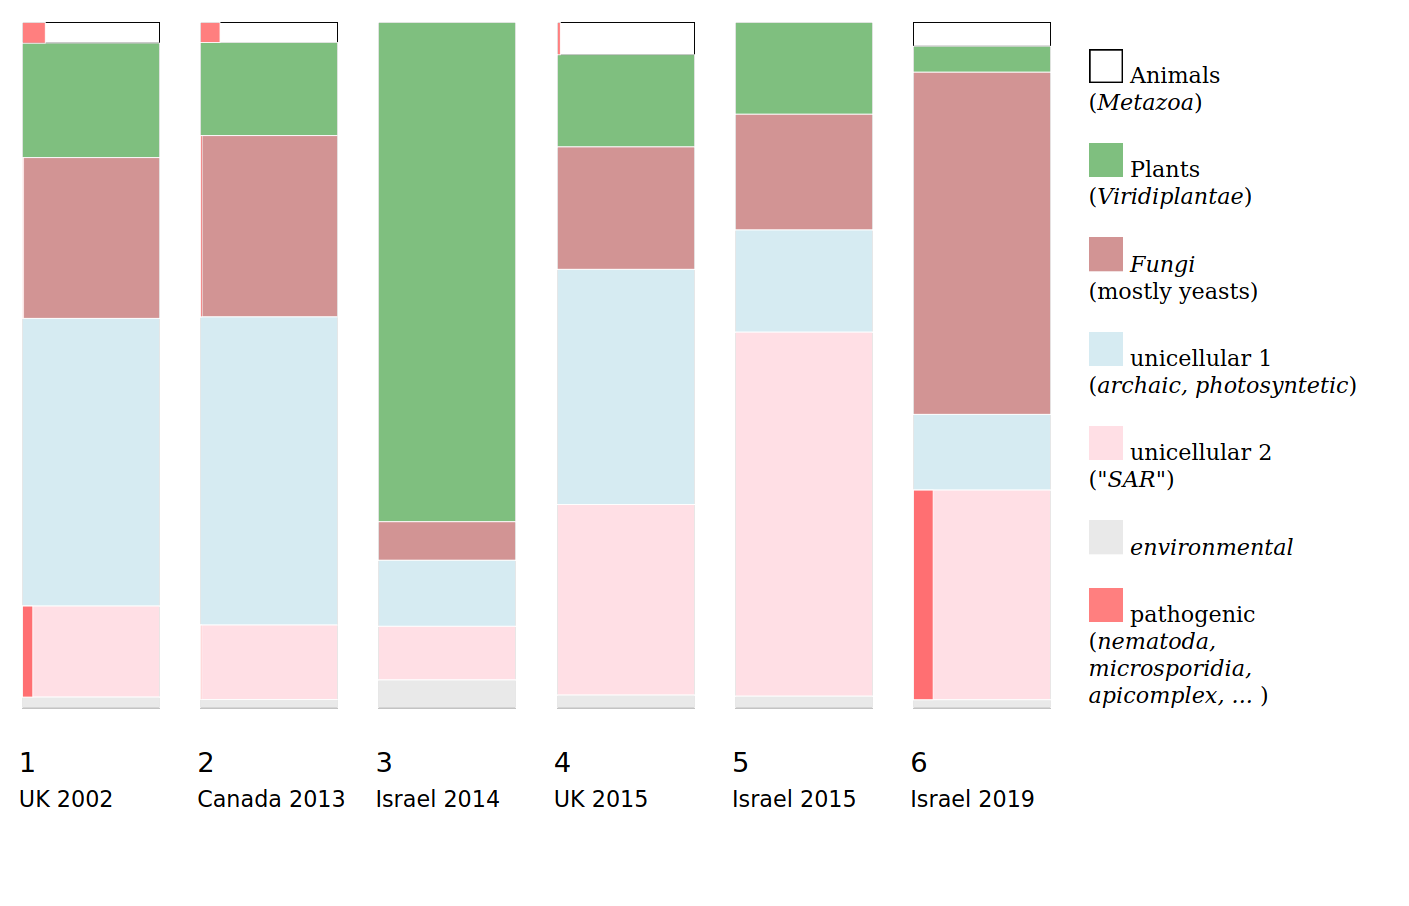
\includegraphics[width=0.99\textwidth]{tilechart.jpg}

Рис. 1 \textit{Соотношение состава групп организмов, по образцам - колонки соответстуют образцам}

Таблица 2.

\begin{tabular}{ll}
\hline
Обозначение&Состав, как характеристика\\
\hline
Animals&\textit{Mollusca,Arthopoda}\\
Plants&\textit{Chlorophyta,Streptophyta}\\
Fungi&95\% - 100\% \textit{Saccharomycotina} (yeast)\\
Unicellular 1&\textit{Euglenozoa,Rhodophyta,Haptophyta,Glaucophyta,Cryptophyta}\\
Unicellular 2&\textit{Cercozoa,Strametopiles,Alveolata}\\
\hline
\end{tabular}

На рисунке выделены красным группы, включающие паразитические организмы, потенциально вызывающие хронические трудно излечимые расстройства здоровья. Это,
в образцах 1,6 - \textit{Nematoda}, в образце 4 - \textit{Platyhelmintes}, паразитические черви; в образцах 1,2, как следы - \textit{Microsporidia}, паразитические организмы, выживающие внутри клеток хозяина, и многоклеточные подобно грибам; в образце 1 - \textit{Apicomplexa}, в образце 6 - \textit{Haplosporida} и следы \textit{Cnidaria} - микроорганизмы, отнесенные к \textit{Alveolata}, для которых характерно многообразие паразитических циклов,

\subsection*{Сравнение ''царств'' по кривым распределения численности}

Так называемые ''распределения численности видов'', в экологии, - по сравнению их формы можно выявить особенности экосистем, хотя из моделей для описания их формы, никакая не универсальна, как это обсуждалось в [1]. Кривые распределения численности для разных групп, по всем образцам совместно, показаны на рис. 2, и то что при этом интересует - как форма кривой соотносится с потенциальной неустойчивостью экосистемы.

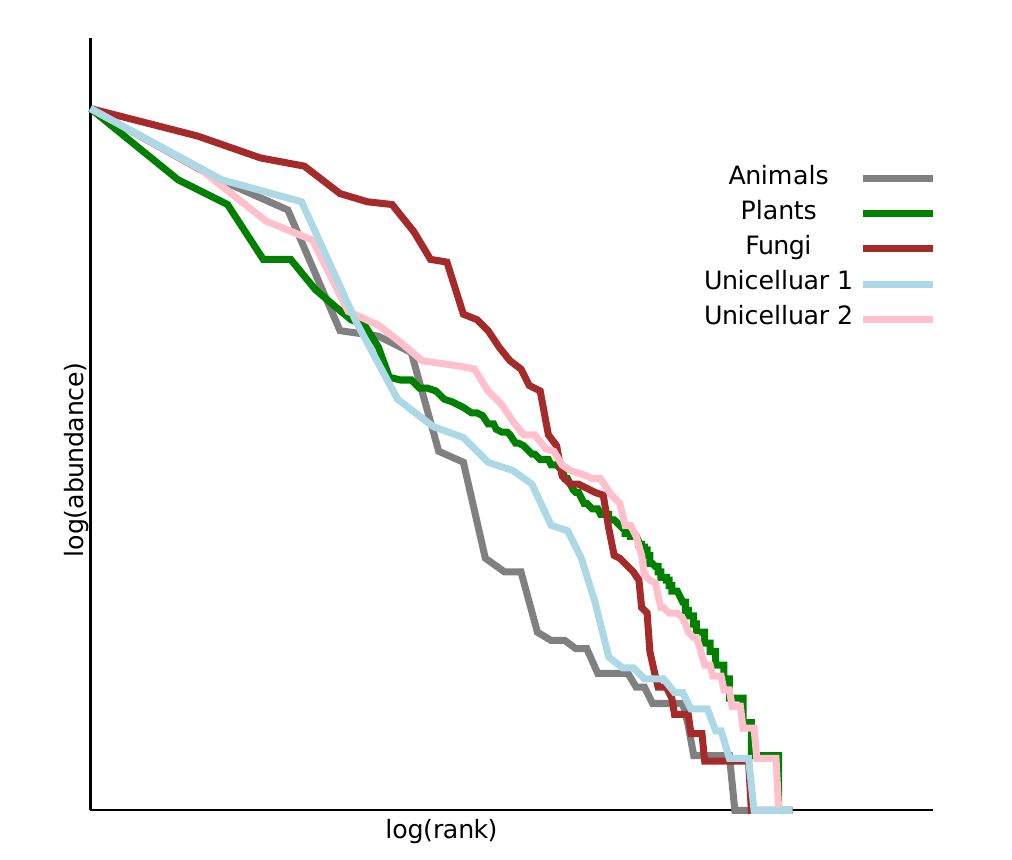
\includegraphics[width=0.7\textwidth]{rankabundance.jpg}

Рис. 2 \textit{Кривые распределения численности, по группам организмов}; 

\subsection*{Интерпретация 1: теоретические модели}

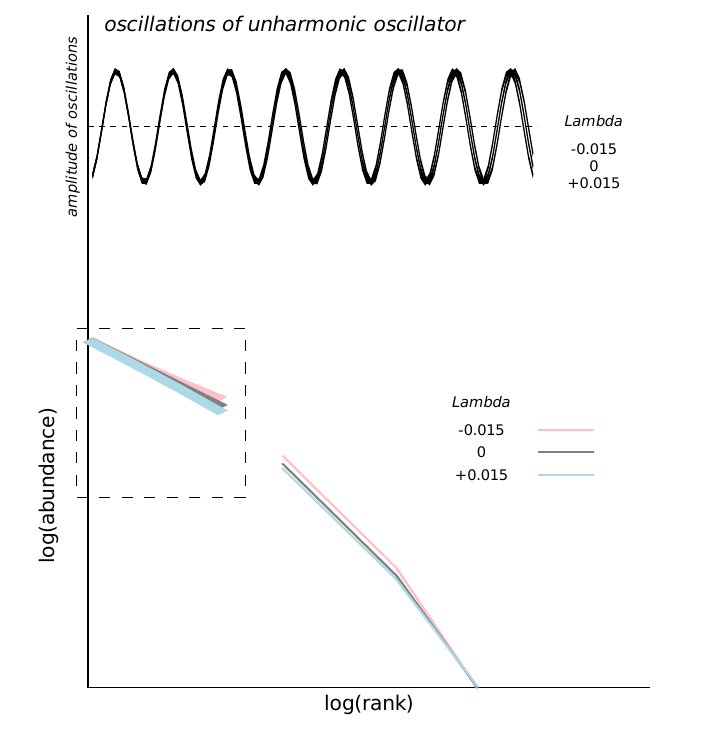
\includegraphics[width=0.7\textwidth]{rankabundance_unharmonic.jpg}

Рис. 3 \textit{смещение частоты колебаний и смещение модельных распределений численности, в модели Ципфа-Парето (обведено рамкой) и модели Больцмана, при разных знаках коэффициента $\lambda$ в ан-гармоническом осцилляторе}

В форме кривых распределения численности, в болшей или меньшей степени, применимы как модель "закона Ципфа-Парето", так и модель распределения Больцмана. Обе модели, которые в других ситуациях применимы вполне явно, выражают соотношение между линейным возрастанием ''энергии'' системы, от уровня к уровню, и экспоненциальным убыванием ''заселенности'' уровней; в распределении Ципфа-Парето ''энергия'' вводится неявно и выражается по логарифмическому закону. 

Сводя вопрос сравнения численности видов к сравнению неустойчивости групп при сменах времен года, месяцев, дней и ночей, сменах дождей и яснй погоды, сменах полноводных паводков на маловодные при разливах рек - то что и определяет избыток питания в экологических нишах и под-группах, и ''заселенность'' в этих нишах - признаки искажения такой периодичности, индуцируимые через обратную связь, были бы признаком неусточивости.

Для минимально простого описания искажений периодичности, подойдет модель осциллятора с малым дополнением, внесенным в закон движения, так что в колебаниях такого ''не-гармонического'' осциллятора проявляются отклонения от гармонического закона - то что может являеться признаком потенциальной неустойчивости.

В квантовом описании, уровни энергии такого осциллятора зависят от квантового числа не вполне линейно. Используя формулу для расчета уровней энергии, предложенную в [2], через поправки к модели Ципфа-Парето и модели Больцмана на рис. 2 показано, как отклонения от периодичности проявлялись бы в кривых распределения видов.

Нарастающая периодичность соответствует положительному знаку в не-гармоничной поправке в модели осциллятора ($\hat H = p^2 + x^2 + \lambda x^4$), замедляющаяся перидичность - отрицательному знаку. Само событие кризиса в этой модели не описывается и не предсказывается. Эмпирически, колебания с нарастающим периодом - это признак риска кризиса [3]. В рамках самой модели квантового ангармонического осциллятора, ''сбой'' его движения возможен при отрицательном $\lambda$, через тоннельный переход в один из двух сегментов с отрицательной энергией за пределами области колебаний.

\subsection*{Интерпретация 2: сравнение с системой регуляции генов}

Для генов, отсортированных по уровню экспрессии, на диаграммах - и как общее правило, и в представленных результатах - отделяется группа генов с высоким уровнем. Для остальных выполняется, в целом или частично, правило Ципфа-Мандельброта, линейная форма зависимости экспрессии от порядкового номера, построенной в логарифмических координатах.

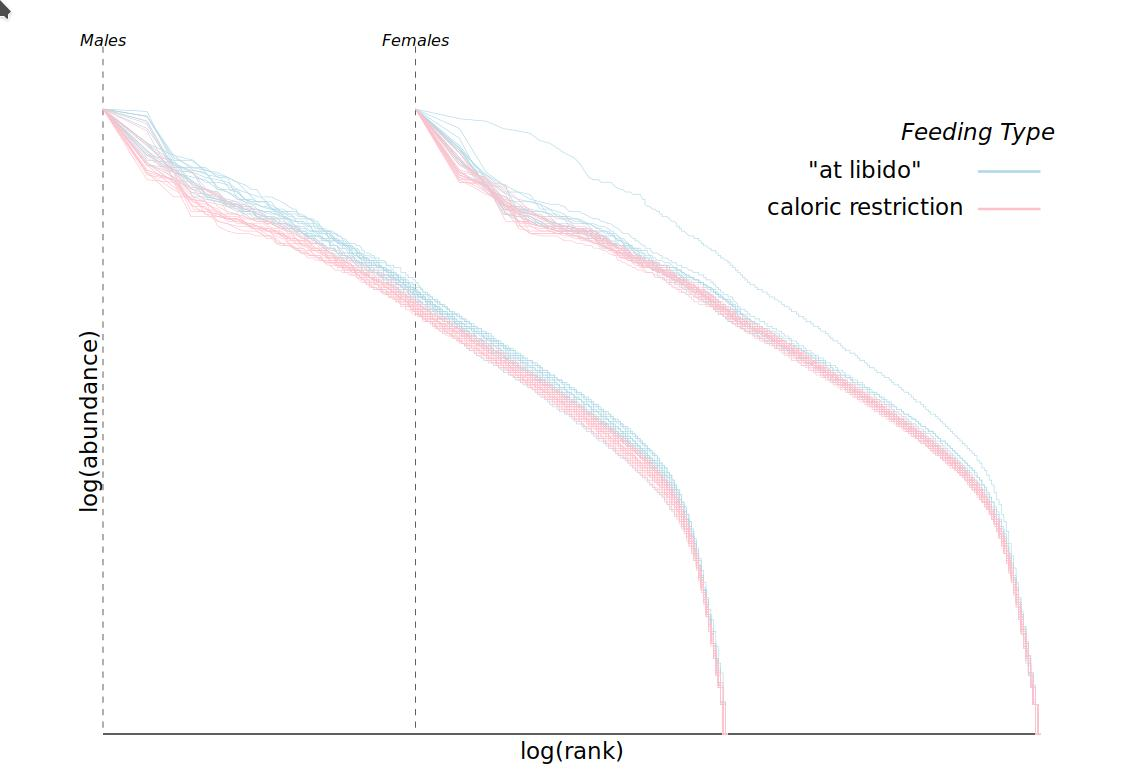
\includegraphics[width=0.85\textwidth]{rankabundance_rnaseq.jpg}

Рис. 4 \textit{Распределение уровней экспрессии генов. розовые линии - мыши на голодном пайке, по сравнению с контролем}

По оценке фрактальной размерности суточного ритма, у самок различие проявляется более заметно, и в противоположном,чем у самцов, направлении:

\begin{tabular}{lll}
\hline
&самцы&самки\\
\hline
голодные&1.00225 &1.00622\\
не голодные&1.00263&1.00108\\
\hline
\end{tabular}

\subsection*{Выводы}

Подводя итоги, отклононения от равновесия, следуя представленным интерпретациям, возмоны в двух направлениях, условно обозначенных ниже А и Б:

А - ускорение циклов и колебаний, то что грозит риском кризиса по типу ''внезапного обвала''. Характерно для самок в поисках еды и самцов, в достаточной степнени сытых.

Б - замедление циклов и колебаний, где риском является ''угасание'' и ''растворение''.

Не говоря о разнообразных группах одноклеточных организмов, про которые мало известно, для трех царст живого направления их отклонения, по диаграммам численности, показны ниже:

\begin{tabular}{lll}
\hline
&многочисленные виды&редкие и малочисленные виды\\
Животные&А&А\\
Растения&А&Б\\
Грибы&Б&А\\
\hline
\end{tabular}

\section{Методы}

Брали образцы где эксперимент был поставлен как полно-геномное секвенирование микробного сообщества, на секвенаторах одной и той же торговой марки. Смотрели на состав сообщества по рибосомной РНК, кроме бактерий у которых эта РНК отличается. Обработку делали в два приема - отбирали из общего пула фрагмены искомой РНК, и аккуратно сравнивали их с базой рРНК организмов, отнесенных каждый к какой-либо такономической категории согласно принятой классиификации.

Ниже указаны формальные характеристики шести использованных образцов:

\begin{tabular}{lllllllll}
\hline
&Sample ID&Bases&Reads&Location&Date&18S RRNAs\\
\hline
1&ERR981203&5.3G&10M&51.83N 0.21E&2002.06.23&1517(*)\\
2&SRR6030929&2.4G&6.1M&42.98N 81.24W&2013&125002(*)\\
3&ERR588716&8.2M&159K&Israel&2014 or earlier&848\\
4&ERR970400&4.2G&13M&51.61N 3.95E&2015.01.01&18747 (*)\\
5&SRR7642476&77M&128K&30.78N 34.76E&2015.08.20&4231\\
6&SRR12806764&48M&97K&31.86N 34.72E&2019.02.25&116666\\
\hline
\end{tabular}

Составление референсной бызы 18S RRNA:

cat ssu\_jan03.tsv | bash -c 'while read line; do if [ ''\$\{line:0:4\}'' == "tax," ]; then if [ ''\$\{line:5:5\}'' == ''Eukar'' ]; then if [''\$f'' == ''2'' ]; then echo ''\$i" ''\$\{line:5\}; i=`echo \$i + 1 | bc`; f=''1''; fi;fi;  else if [ ''\$f'' == ''1'' ]; then if [ ''\$\{line:5\}'' != '''' ]; then echo \$\{line:5\}; f=''2''; fi; fi; fi; done; ' | awk '\{ if ( \$2 == ''Eukaryota;'' || ( p == ''Eukaryota;'' \&\& length( \$0 ) > 100 ) ) \{ print \$0 \}; p = \$2 \}' | awk '\{ if ( p != \$2 ) \{ print \$0 \}; p = \$2 \} ' >rrna\_euk.fa

cat \$sample | awk '\{ print substr( \$1, 1, length( \$1 ) - 1 ) \}' | bash -c 's='''';c=0;while read line; do if [ ''\$line'' != ''\$s'' ]; then if [ ''\$s'' != '''' ]; then echo ''\''\$s\'' : \$c,''; fi; s=\$line; c=1; else c=`echo ''\$c+1'' | bc`; fi; done;

sort \$sample |  bash -c 's='''';c=0;while read line; do if [ ''\$line'' != ''\$s'' ]; then if [ ''\$s'' != '''' ]; then echo ''\$s \$c''; fi; s=\$line; c=1; else c=`echo ''\$c+1'' | bc`; fi; done;' | awk '\{ print \$3 '' '' \$(NF-1) '' '' \$NF \}' | sort - | bash -c 's='''';b='''';c=0;while read line; do if [ ''\$\{line:0:5\}'' != ''\$\{s:0:5\}'' ]; then h=`echo \$s |awk '''''''\{print \$1\}'''''''`; echo ''\$h \$b''; c=0; s=\$\{line\}; else n=`echo \$line | awk '''''''\{print \$NF\}'''''''`; if [ \$n -gt \$c ]; then c=\$n; b=`echo \$line | awk '''''''\{ print \$(NF-1) \}'''''''`; fi; fi; done; h=`echo \$s |awk '''''''\{print \$1\}'''''''`; echo ''\$h \$b'''

Обработка образцов:

head -n 4000000 \$sample.fastq >t0.fastq

sortmerna --ref ssu.fa,ssu.idx --reads t0.fastq --aligned t1 --sam

cat t1.sam | awk '{ print ''>'' \$1 ''\\n'' \$10 }' > t2.fa

blastn -db ssu.db -query t2.fa -evalue 1e-2 -task blastn -max\_target\_seqs 1 -out t3.tsv -outfmt ''6 sallseqid''
out=test-\${sample}

mv \${out}.tsv t3.tsv

cat t3.tsv | while read line; do t=`grep ''>\$line '' ssu.fa`; echo \${t:1} >>\$out.txt; done;

cat \$out.txt | awk '{ gsub(/[0-9]/,''''); gsub( ''; '', '','' ); print }' | sort >\${out}.csv

cat \$out.csv | awk -F '','' '{ print \$2 '' '' \$3 }' | bash -c 's='''';c=0;while read line; do if [ ''\$line'' != ''\$s'' ]; then if [ ''\$c'' != ''0'' ]; then echo ''  \''\$s\'' : \$c,''; fi; s=\$line; c=1; else c=`echo ''\$c+1'' | bc`; fi; done; echo ''  \''\$s\'' : \$c'';'; 

 

Таблица 3: \textit{Количество аннотированных фрагментов рРНК по группам в каждом из образцов}

\begin{tabular}{lllllll}
\hline
Taxonomy(*) &1&2&3&4&5&6\\
\hline
Acanthamoebidae Acanthamoeba&2&4& &1& &\\
Alveolata Apicomplexa&12&&&14& &\\
Alveolata Ciliophora&&&&2&9&1\\
Alveolata Haplosporida&&4&&&&5406\\
Cercozoa Cercomonadida&&2&&&&\\
Cercozoa Chlorarachniophyceae&4307&197&5&108&876&14637\\
Cryptophyta Cryptomonadaceae&91&&&9&389&382\\
Cryptophyta Teleaulax&&2&&&&\\
Diplomonadida Hexamitidae&19&5&&2&&\\
environmental samples&357&50&35&25&1206&1490\\
Euglenozoa Euglenida&407&84&&46&&1\\
Euglenozoa Kinetoplastida&2072&785&4&270&1206&5343\\
Fungi Ascomycota&3343&1044&&347&11860&60992\\
Fungi Basidiomycota&&&48&3&4&\\
Fungi Chytridiomycota&&&&1&&\\
Fungi Microsporidia&1&12&&3&2&12\\
Fungi Zygomycota&5&8&&&1&\\
Glaucocystophyceae Glaucocystales&77&56&&12&2890&5020\\
Glaucocystophyceae Gloeochaetales&244&8&8&9&5042&1845\\
Granuloreticulosea Foraminifera&3&&&&&\\
Haptophyceae Isochrysidales&317&103&11&24&33&19\\
Haptophyceae unclassified Haptophyceae&17&2&&1&32&24\\
Metazoa Acanthocephala&&&&&&1\\
Metazoa Arthropoda&382&12&&13&2424&627\\
Metazoa Chordata&&2&&5&&\\
Metazoa Cnidaria&&&&&&6\\
Metazoa Mollusca&475&91&&22&8907&3641\\
Metazoa Myxozoa&&&&8&&2\\
Metazoa Nematoda&&15&&&&38\\
Metazoa Platyhelminthes&26&&&&&13\\
Metazoa Porifera&&&&&6&\\
Parabasalidea Trichomonadida&2&&&1&&\\
Rhodophyta Bangiophyceae&2962&541&43&175&714&801\\
Rhodophyta Florideophyceae&232&227&16&88&148&110\\
stramenopiles Bacillariophyta&125&47&3&10&3091&312\\
stramenopiles Chrysophyceae&41&10&1&1&3&3\\
stramenopiles Olisthodiscus&379&29&&17&28&78\\
stramenopiles Oomycetes&&2&&&&\\
stramenopiles Phaeophyceae&33&6&&&1&\\
stramenopiles Placididea&303&136&57&48&33139&17046\\
Viridiplantae Chlorophyta&1636&401&478&139&1563&2569\\
Viridiplantae Streptophyta&876&315&137&113&7886&4583\\
\hline
\end{tabular}

{\small(*) Таксономия согласно версии EBI, 2-й и 3-й уровни.}

Кривые численности: 

e.g, SAR:

grep -E 'Cercozoa|strametopiles|Alveolata|Acanthamoeba' test*.txt | sort | awk '\{ print \$1 \}' |  bash -c 's='''';c=0;while read line; do if [ ''\$line'' != ''\$s'' ]; then if [ ''\$s'' != '''' ]; then echo \$c; fi; s=\$line; c=1; else c=`echo ''\$c+1'' | bc`; fi; done; echo \$c' | sort -g | awk '\{ s = \$0 '' '' s \} END \{ print s \}' | awk '\{ s = ''''; for ( i=1; i <= NF; i++ ) \{ s = s '' '' log(i)/log(NF) '','' log(\$i)/log(\$1) \}; print s \}'

Unharmonic oscillator

classical system:
{\texttt \small
awk '\{ lambda=\$1; x = 1; v = 0; dt = 0.01; s = ''''; for ( i = 1; i < 5000; i++ ) \{ x = x + v * dt; v = v - x * ( 1 + lambda * x * x ) * dt; if ( i \% 50 == 0 ) \{ s = s '' '' ( i * dt ) '','' x; \}; \}; print s \}' 
}

C code:

{\texttt \small
void solve\_cubic( double h, double g, double *e1 ) \{ double d = atan2( sqrt( pow( h, 3 ) - g * g ), -g ) / 3.;   double c = sqrt( h ) * cos( c );  *e1 = 2 * c; \}

    
int main( int argc, char **argv ) 
\{  
    double lambda = atof( argv[1] );
    double nmax = atoi( argv[2] );
    double omega\_n;    
    int n;
    for ( n = 0; n < nmax; n++ )
    \{
        solve\_cubic( 1. / 3., -3. * lambda * ( 1. + 2. * n + 2. * n * n ) / ( 1. + 2. * n ), \&omega\_n );
        printf( ''\%.2f '', ( 1. / 4. ) * ( 3. * omega\_n + 1. / omega\_n )* ( n + 1. / 2 ) );

    \}
 \}
}
 
Rna-seq

rank-abundance

for ft in FAL MAL FCR MCR; do for cn in 28 29 30; do cat RNAseq\_WT\$ft.csv | awk -F "," -v cn=\$cn -v i=0 '\{ if ( \$cn > 0 \&\& i > 0 ) print \$cn; i = i + 1 \}' | sort -g -r | awk -v sname="'"\$ft\$cn"'" 'BEGIN \{ print sname ":["; s = ""; i = 0 \} \{ i = i + 1; if ( ( i \% 20 ) == 0 ) \{ print s ","; s = \$1 \} else \{ if ( i > 1 ) \{ s = s "," \$1; \} else \{ s = \$1 \} \}; \} END \{ print s "]," \}' >>rnase\_distributions.txt; done; done;

fractal dimension:

{\texttt \small
awkcmd='\{ n1 = abs( \$1 - \$2 ) + abs( \$2 - \$3 ) + abs ( \$3 - \$4 ) + abs(  \$4 - \$5 ) + abs( \$5 - \$6 ); n2 = 0.5 * ( abs(  \$1 - \$3 ) + abs( \$2 - \$4 ) +  abs(  \$3 - \$5 ) + abs( \$4 - \$6 ) ); n3 = 0.3333 * ( abs(  \$1 - \$4 ) + abs( \$2 - \$5 ) + abs( \$3 - \$6 ) ); l2 = log(2 ); l3 = log( 3 );  if ( n1 > 0 \&\& n2 > 0 \&\& n3 > 0 ) \{ y = log( n1 ) + log( n2 ) + log( n3 ); b = ( 3 * ( log( n3 ) * l3 + log( n2 ) * l2 ) - y * 1.79 ) / 1.84; a = ( y - b * 1.79 ) / 3; d1 = log( n1 ) - a; d2 = log( n2 ) - a -b * l2; d3 = log( n3 ) - a - b * l3; sumd = d1 * d1 + d2 * d2 + d3 * d3; if ( sumd < 0.01 ) \{ print abs(b) \} \}  \} function abs( v ) \{ if ( v > 0 ) \{ return v; \} else \{ return -v; \} \}'

fdim=`awk ''\$awkcmd'' | sort -g | head -n \$median | tail -n 1`
}

\section{References}

\begin{enumerate}

\item Feranchuk, S., Belkova, N., et al., Evaluating the use of diversity indices to distinguish between microbial communities with different traits. Res. Microbiol., 2018

\item Feranchuk, I., Komarov, L., et al., Operator method in the problem of quantum unharmonic oscillator, Annals of Phys., 1995 

\item Nottale, L., Scale relativity and fractal space-time: theory and applications, arxiv.org, 2008

\end{enumerate}

\end{document}
